\documentclass[a4paper, 12pt, titlepage]{article}
\usepackage{a4wide}
\usepackage{amsmath}
\usepackage[pdftex]{graphicx}
\usepackage{pdfpages}
\usepackage{subcaption}
\usepackage{listings}
\usepackage{color}
\usepackage{cite}
\usepackage{import}
\usepackage[title,titletoc,toc]{appendix}

\title{Multirotor Drone Collision Avoidance}
\author{Richard Allen}

\begin{document}

\begin{titlepage}
    \begin{center}
        % Upper part of the page. The '~' is needed because \\
        % only works if a paragraph has started.
        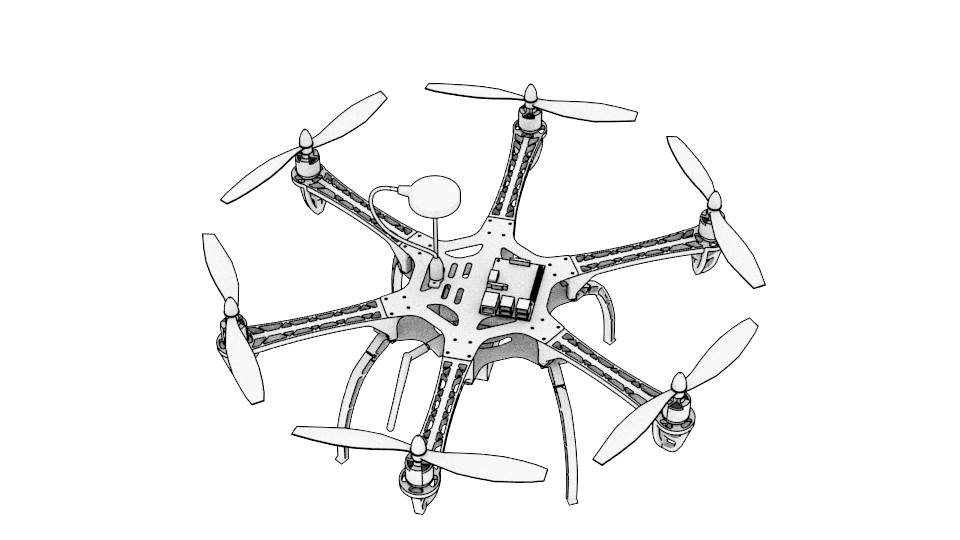
\includegraphics[width=0.7\textwidth]{./logo.jpg}~\\[1cm]
        \textsc{\Large Final Year Project Proposal}\\[0.5cm]
        % Title
        %\HRule \\[0.4cm]
        { \huge \bfseries Multirotor Drone Collision Avoidance \\[0.4cm] }
        %\HRule \\[1.5cm]
        % Author and supervisor
        \noindent
        \begin{minipage}[t]{0.4\textwidth}
        \begin{flushleft} \large
        \emph{Author:}\\
        Richard \textsc{Allen}
        \end{flushleft}
        \end{minipage}%
        \begin{minipage}[t]{0.4\textwidth}
        \begin{flushright} \large
        \emph{Supervisors:} \\
        Prof.~Thomas \textsc{Braunl}\\
        Chris \textsc{Croft}
        \end{flushright}
        \end{minipage}
        \vfill
        % Bottom of the page
        {\large \today}
    \end{center}
\end{titlepage}



%\maketitle

\begin{abstract}
    This report outlines a study into adapting an unmanned aerial vehicle for autonomous control. The main focus of study is on collision avoidance on widely accessible platform with relatively limited computing power. 
    It includes: 
    \begin{itemize}
        \item An overview of the platform hardware and design choices in it's construction,
        \item An explanation of the data structures used for storing and navigating around obstacles in the environment, and
        \item An explanation of the algorithms used for navigation.
    \end{itemize} 
\end{abstract}

\tableofcontents
\newpage

\section{Introduction}
	\subsection{Motovation}
The average person's environment has never had more autonomy. This trend will only continue as more of our infrastructure moves into the domain of mechatronics engineering. Already we have widespread adoption of networked computers for personal use as well as in autonomous systems. Now with projects such as driverless cars, the trend is extending to robots that must deftly navigate complex and uncontrolled human environments.
Drones themselves are seeing application in the sciences, photography, sports, agriculture, search-and-rescue, as well as many other fields. For these purposes, there is increasing need for robust auonomous behaviours.
Enter the events of recent history: The Edward Snowden leaks, as well as the Volkswagen emissions testing scandle have demonstrated the degree of power now in the hands of mechatronics engineers. That power has been thrown into sharp relief by demonstrations of its abuse.

	\subsection{Project History}
		\subsubsection{2013}
		\subsubsection{2014}

\section{Background}
    \subsection{Obstacle detection methods}
        \subsubsection{LIDAR}
        \subsubsection{Optical Flow}
        \subsubsection{Stereoscopy}
        
\section{Design}
    \subsection{Picopter}
    \subsection{ArduPilot}
    \subsection{Software design}
    \subsection{Web interface}
    \subsection{Obstacle navigation}
        \subsubsection{graph data structure}
        \subsubsection{Astar algorithm navigation}
        \subsubsection{DistBug algorithm navigation}
        \subsubsection{Voronoi graph navigation}
    \subsection{Obstacle detection}
        \subsubsection{LIDAR}
        \subsubsection{Voxel space}

\section{Results}
    \subsection{Astar obstacle avoidance}
    \subsection{voxel space}
        
        
\end{document}    
